\normalsize

\tikzstyle{Line} = [line width=.75pt]
\newcommand{\com}{\operatorname{com}}
% \setcounter{page}{25}
% \normalsize\setcounter{equation}0\setcounter{page}{25}
\baselineskip11.7pt plus.2pt minus.3pt
%\fontsize{10.5}{13}\selectfont
%\advance\parskip by-1pt
%\small
\kpospis{Dla jakich $n$ istnieje\ldots ?}
{Bartłomiej Bzdęga}



\wtyt{Dla jakich $n$ istnieje\ldots ?}

\waut{Bartłomiej BZDĘGA}
{\hfill\scriptsize\rm Uniwersytet im. A. Mickiewicza w~Poznaniu}

%TU SIĘ ZACZYNA MARGINES, CZYLI LOGO, A POTEM WSKAZÓWKI
\marg[-55]
{\centerline{\setbox0=\hbox{\includegraphics[width=3.8cm]{kmo_logo_krzywe}}\copy0\lower.5pt\llap{%
      
\begin{tikzpicture}
        \draw[magenta,line width=3pt] (0,0) circle (1.835);
        \draw[magenta,line width=1pt] (0,0) circle (1.73);
        \draw[magenta,line width=.6pt] (0,0) circle (1.27);
        \draw[magenta,line width=1.3pt] (0,0) circle (1.19);
      \end{tikzpicture}%
    }\raise53pt\llap{\hbox to\wd0{\hss\Large\textbf{\textsf{\textcolor{white}{73}}}\hss}}}

\vskip6.3cm

\medskip


%----WSKAZÓWKI----
\vskip1cm

  \rotatebox{180}
{\vrule~\vbox{\advance\baselineskip by.3pt\textbf{Wskazówki do zadań}
    \medskip
    
   \begin{enumerate}[format=\Magenta,itemsep=0pt,leftmargin=0pt,itemindent=12pt,labelwidth=6pt,labelsep=6pt,itemsep=2pt]
\item Każde dwa sąsiednie boki są prostopadłe, więc $n\ge4$ musi być parzyste.
\item Liczba $1+2+\ldots+2n=n(2n+1)$ musi być parzysta, więc liczba $n$ również.
\item Liczba krawędzi takiego wielościanu jest równa $\frac32n$, więc $n$ musi być parzyste. Dla $n=4$ mamy czworościan foremny, a~dla parzystych $n>4$ można skleić podstawami dwa przystające prawidłowe ostrosłupy $(n/2)$-kątne.
\item Zauważmy, że analogiczna konstrukcja na płaszczyźnie jest wykonalna dla każdego nieparzystego $n$. Jeśli $n=4k+1$, to jako środkową warstwę sześcianu bierzemy konstrukcję z~płaszczyzny, a~dodatkowo z~góry i~z~dołu dokładamy prostopadłościany $n\times n\times 2k$. W~przypadku $n=4k+3$ kolorujemy sześciany jednostkowe sześcianu $n\times n\times n$ w~czarno-białą szachownicę. Niech środkowy sześcianik będzie czarny -- wśród pozostałych jest wtedy więcej białych niż czarnych, z~czego można wywnioskować, że konstrukcja jest niewykonalna.
\item Niech $s_k=x_1+x_2+\ldots+x_k$. Po podniesieniu danej w~zadaniu równości obustronnie do kwadratu, zsumowaniu stronami dla $k=1,2,\ldots,n$ i~prostych przekształceniach otrzymamy $2s_n+n+1 = (x_n+1)^2$, więc $s_n=0 \iff |x_n+1|=\sqrt{n+1}$. Wnioskujemy stąd, że $n=m^2-1$ dla pewnego naturalnego $m$. Osiągalności dowodzimy indukcyjnie, rozważając wszystkie możliwe wartości $x_n$.
\item Liczba $\frac12n^2(n+1)$ musi być kwadratem, więc $n=2k^2-1$ dla pewnej
liczby całkowitej $k$, a~stąd bok kwadratu ma długość $kn$. W~celu wykonania konstrukcji można ułożyć $k^2$ kwadratów $n\times n$.
\item Znana jest mi konstrukcja dla $n=1,2,3,4$ i~nic więcej.
\end{enumerate}
}}}%
% ARTYKUŁ
Zajmiemy się tu zadaniami, w~których należy wyznaczyć wszystkie liczby naturalne
$n$, dla których istnieje pewien zadany obiekt. Trzeba pamiętać, że rozwiązanie takiego
zadania składa się z~dwóch części:
\begin{itemize}
\item w~przypadku tych $n$, dla których dany obiekt istnieje, wystarczy podać jego konstrukcję albo (co się zdarza w~trudniejszych zadaniach) udowodnić jego istnienie metodami pośrednimi, takimi jak na przykład zasada szufladkowa;
\item dla tych $n$, dla których nie istnieje dany obiekt, trzeba przeprowadzić dowód jego nieistnienia, najczęściej metodą nie wprost -- przez założenie istnienia i~doprowadzenie do sprzeczności.
\end{itemize}
Zwykle jedna z~tych dwu części jest łatwiejsza. Pozwala to postawić odpowiednią hipotezę, co często ułatwia rozwiązanie trudniejszej części, ponieważ wiemy już, co chcemy wykazać.\par

Jako przykład rozwiążemy następujące zadanie z~VII Wielkopolskiej Ligi Matematycznej.\par

\textbf{Przykład.} Nazwijmy \emph{grubym} prostokąt o~bokach $x$ i $y$ spełniających warunek $\frac12x < y<2x$. Wyznaczyć wszystkie liczby naturalne $n$, dla których z~kafelków o~wymiarach $1\times1, 1\times2, \ldots, 1\times n$ można ułożyć gruby prostokąt (każdy z~kafelków musi być użyty dokładnie jeden raz).\par

\emph{Rozwiązanie.} Pole takiego prostokąta jest równe $\frac12n(n+1)$, dodatkowo jeden z~boków ma długość co najmniej $n$. W~takim razie drugi bok ma długość co najwyżej $\lfloor\frac12(n+1)\rfloor$, co jest równe $\frac12n$ dla $n$ parzystych. Ale wówczas otrzymany prostokąt nie jest gruby. Udowodniliśmy zatem, że dla parzystych $n$ taki prostokąt nie istnieje. \par

\smallskip
\begin{minipage}{\textwidth}
\begin{minipage}{6cm}
W~przypadku nieparzystych $n$ możemy skonstruować gruby prostokąt, tak jak na rysunku obok.
\end{minipage}\hspace*{.5cm}
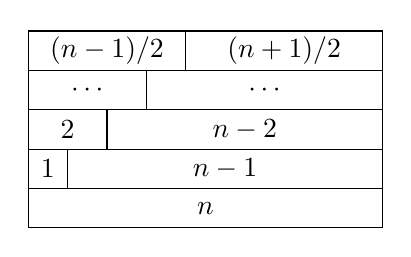
\begin{tikzpicture}[baseline={([yshift={-17pt}]current bounding box.north)}]
\foreach \Y in {0,0.5,1,1.5,2,2.5} {\draw (0,\Y)--(4.5,\Y); }
\foreach \Y in {0.5,1,1.5,2} {\draw (\Y,\Y)--(\Y,\Y+0.5);}
\draw (0,0)--(0,2.5); \draw (4.5,0)--(4.5,2.5);
\node at (0.25,0.75) {$1$}; \node at (0.5,1.25) {$2$}; \node at (0.75,1.75) {$\cdots$}; \node at (1,2.25) {$(n-1)/2$};
\node at (2.25,0.25) {$n$}; \node at (2.5,0.75) {$n-1$}; \node at (2.75,1.25) {$n-2$}; \node at (3,1.75) {$\cdots$}; \node at (3.25,2.25) {$(n+1)/2$};
\end{tikzpicture}
\end{minipage}\par\medskip

Widoczny tu motyw parzystości często pojawia się w~tego typu zadaniach.\par


\textbf{Zadania}
\begin{enumerate}[widest=1,itemsep=0pt]
\item Wyznaczyć wszystkie liczby naturalne $n\ge4$, dla których istnieje $n$-kąt, którego każdy kąt wewętrzny ma $90^\circ$ lub $270^\circ$.
\item Dla jakich liczb całkowitych dodatnich $n$ zbiór $\{1,2,3,\ldots,2n\}$ można rozbić na dwa rozłączne $n$-elementowe podzbiory o~jednakowych sumach?
\item Wyznaczyć wszystkie liczby naturalne $n$, dla których istnieje $n$-ścian wypukły, którego wszystkie ściany są przystającymi trójkątami.
\item Niech $n$ będzie liczbą nieparzystą. Z $\frac{n^3-1}2$ niebieskich
prostopadłościanów o~wymiarach $1\times1\times2$ i~jednego zielonego o~wymiarach
$1\times1\times1$ chcemy zbudować sześcian o~krawędzi $n$, ale środek powstałego
sześcianu ma leżeć w~środku zielonego klocka. Wyznaczyć wszystkie $n$, dla
których jest to możliwe.  \item Znaleźć wszystkie całkowite dodatnie $n$, dla
których istnieje ciąg $(x_0,x_1,\ldots,x_n)$ o~następujących własnościach:
$x_0=0$, $x_1+x_2+\ldots+x_n=0$ oraz $|x_k|=|x_{k-1}+1|$ dla każdego
$k=1,2,\ldots,n$. (LII OM, zmodyfikowane)
\item Wyznaczyć wszystkie dodatnie liczby całkowite $n$ o~następującej własności: z $n$ prostokątów o~wymiarach $1\times n, 2\times n, \ldots, n\times n$ można ułożyć kwadrat. (LXXV OM)
\end{enumerate}

\textbf{Problem otwarty}
\begin{enumerate} \setcounter{enumi}6
\item {\spaceskip.33em minus.17emNa płaszczyźnie znaduje się $n$ punktów czerwonych, $n$ zielonych i~$n$~niebieskich.} Każda prosta przechodzi albo przez co najwyżej jeden z~tych punktów, albo przez dwa punkty jednakowego koloru, albo przez trzy punkty różnych kolorów. Wyznaczyć wszystkie możliwe wartości $n$. (Problem autorski, częściowe rozwiązanie w~Matematycznym Kalendarzu Adwentowym 2021).
\end{enumerate}



\eject